\newif\ifvimbug
\vimbugfalse

\ifvimbug
\begin{document}
\fi

\exercise{Linear Regression}

In this exercise, you will use the dataset \texttt{linRegData.txt}, containing $150$ points in the format \texttt{<input variable, output variable>}. The input is generated by a sinusoid function, while the output is the joint trajectory of a compliant robotic arm. 
The first 20 data points are the training set and the remainder are the testing set.

\begin{questions}

%----------------------------------------------

\begin{question}{Polynomial Features}{10}
Write the equation of the model and fit it with polynomial features. Using the Root Mean Square Error (RMSE) as a metric for the evaluation, select the complexity of the model (up to a 21st degree polynomial) by evaluating its performance on the testing data. Which is the best RMSE you achieve and what is the model complexity? Does it change if we evaluate our model on the training data? Comment your findings and plot the RMSE for each case (use two lines, one for evaluation on training data, one for evaluation on testing data).
For the estimation of the optimal parameters use a ridge coefficient of $\lambda=10^{-6}$.
\\Using what you think is the best learned model from the previous point, show in a single plot the ground truth (full dataset) and the model prediction over it.
Attach snippets of your code showing how you generate polynomial features and how you fit the model.

\begin{answer}
\end{answer}
First we plot the whole ground truth to get a look at our dataset.
\begin{figure}[H]
	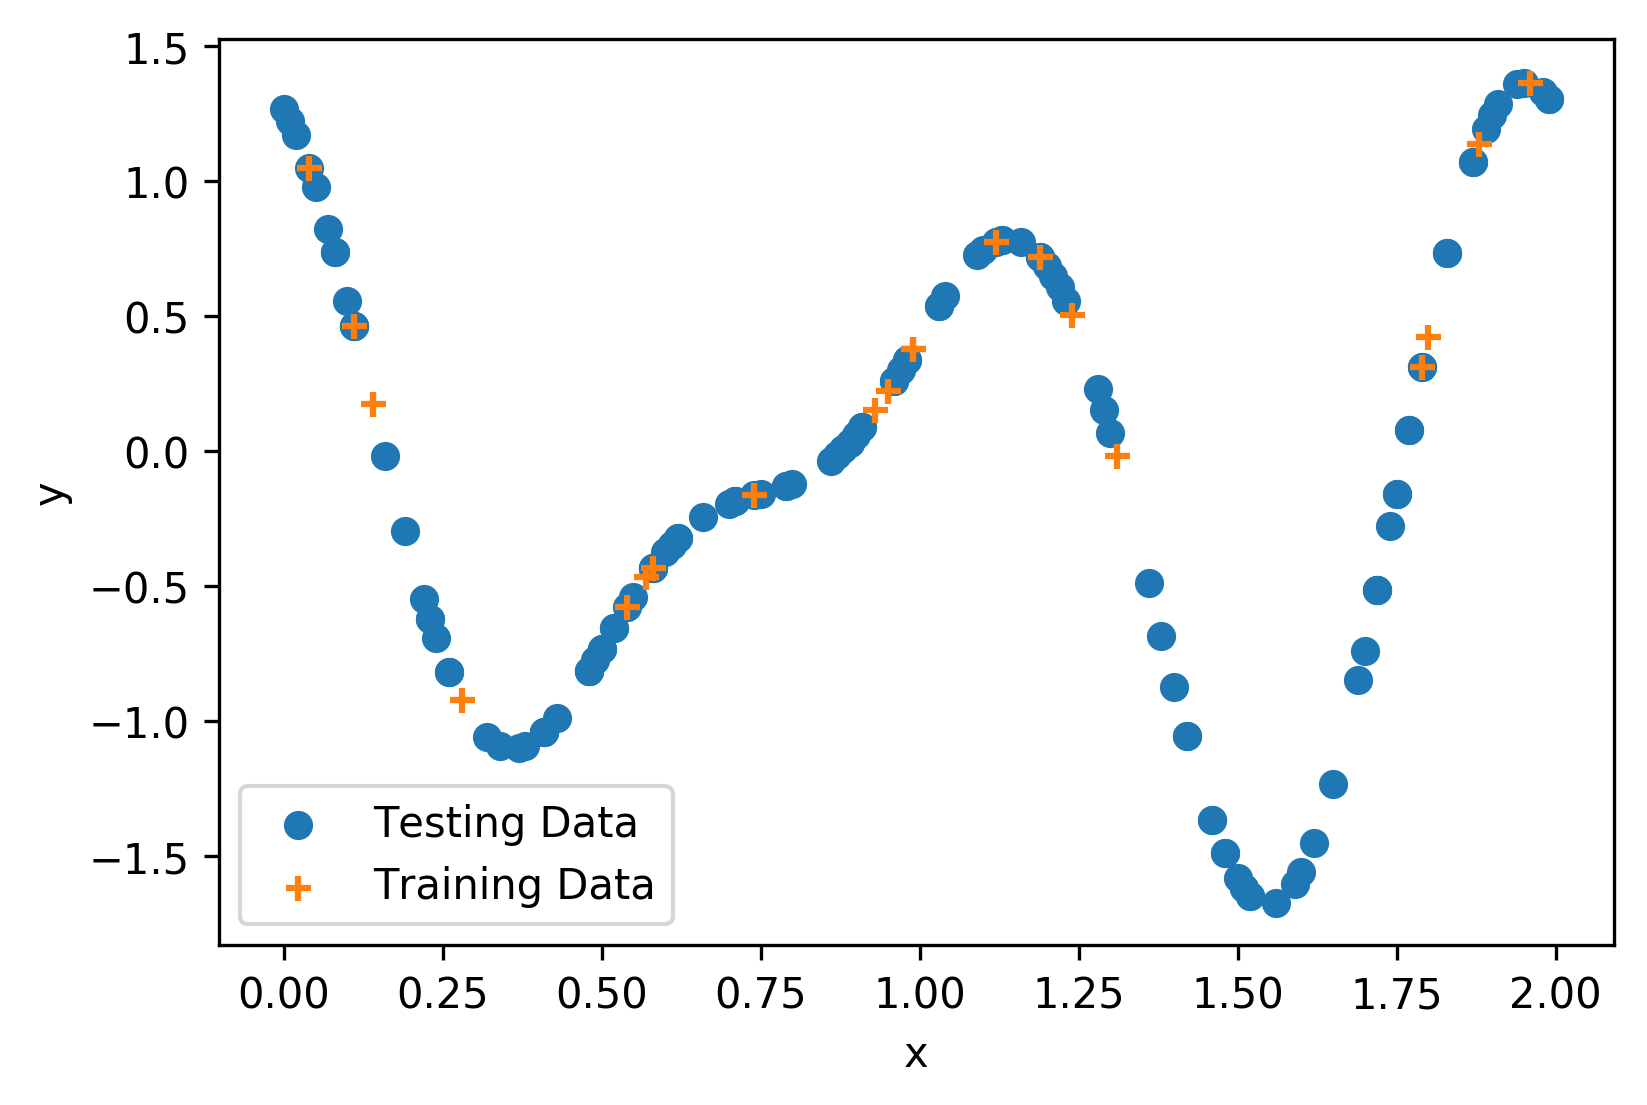
\includegraphics[width=0.6\linewidth]{pictures/groundTruth.png}
	\centering
	\caption{Plotting the whole dataset}
	\label{fig:ground Truth}
\end{figure}

Now that we had a look into the data, let's try our polynomial regression with varrying degree. Interesingly we found two different way to calculate our regression based on numericall differences in numpy. We will talk more about this later, but first lets look at the results.
\begin{figure}[H]
	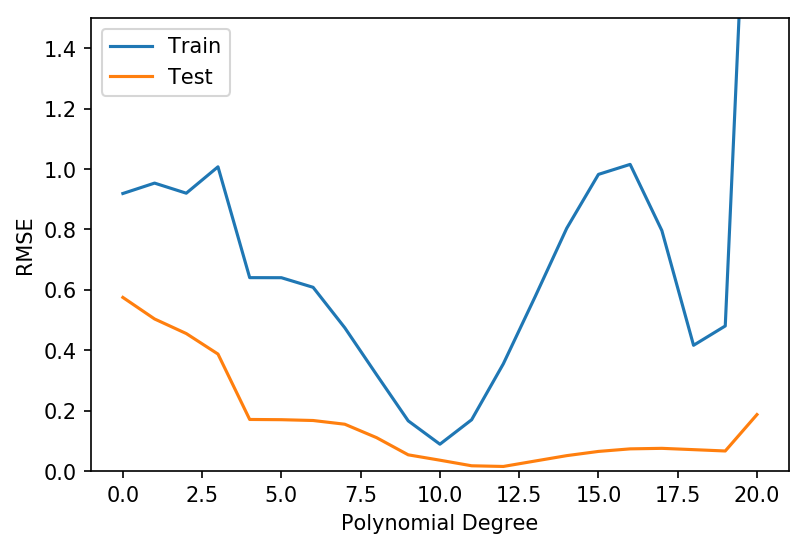
\includegraphics[width=0.6\linewidth]{pictures/polynomial_regression_ridge.png}
	\centering
	\caption{Plotting the error for all different Polynomials using the given ridge coefficient. The minimum lies at degree 10 (RMSE=0.08899).}
	\label{fig:ridge}
\end{figure}
Lets have a look at the actual predictions given by this model.
\begin{figure}[H]
	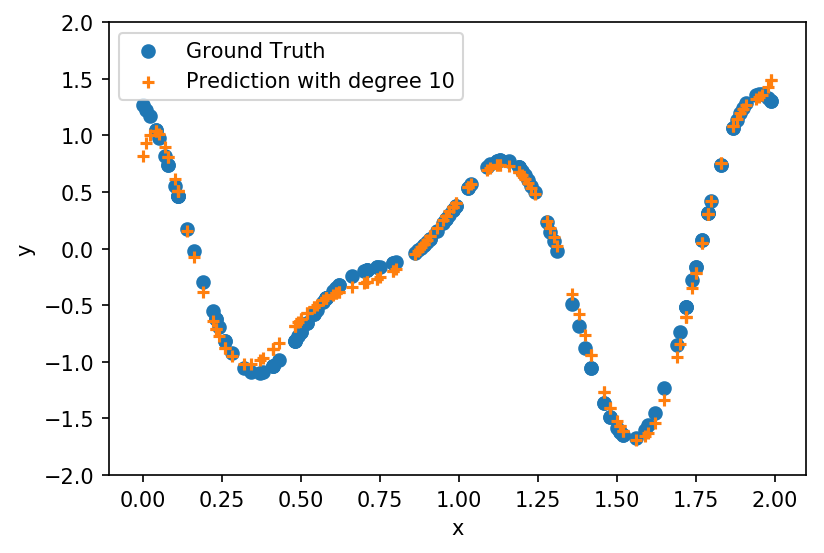
\includegraphics[width=0.6\linewidth]{pictures/groundTruth_polynomial_10.png}
	\centering
	\caption{The dataset and the predictions by our model.}
	\label{fig:pred_10}
\end{figure}

However while working on this task, we found a different way to calculate the pseudo inverse. Instead of multiplying all the different matrixes and adding the ridge coefficient we also tried the numpy function \textit{pinv} to calculate the pseudo inverse directly. The method uses singular value decomposition (SVD) to calculate the pseudo inverse and also cuts small values in the diagonal matrix off. This leads to far better results.
 \begin{figure}[H]
 	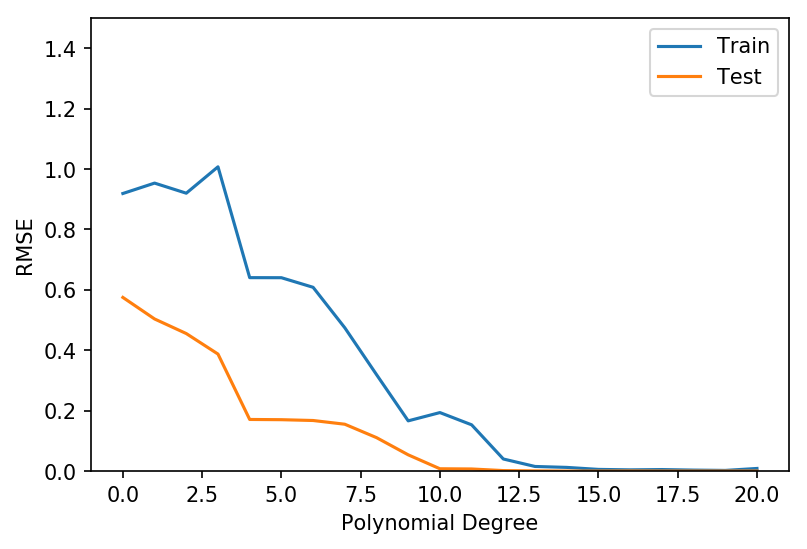
\includegraphics[width=0.6\linewidth]{pictures/polynomial_regression_our_version.png}
 	\centering
 	\caption{Plotting the error for all different Polynomials using np.linalg.pinv for the pseudo-inverse. The minimum lies at degree 21 (RMSE=0.00491).}
 	\label{fig:pinv1}
 \end{figure}
This plot \ref{fig:pinv1} only has a single problem. It doesn't tell us when to start overfitting, so there might be the possibility of even better results if we extend the scope of the task to higher polynomials up to degree 25.
 \begin{figure}[H]
	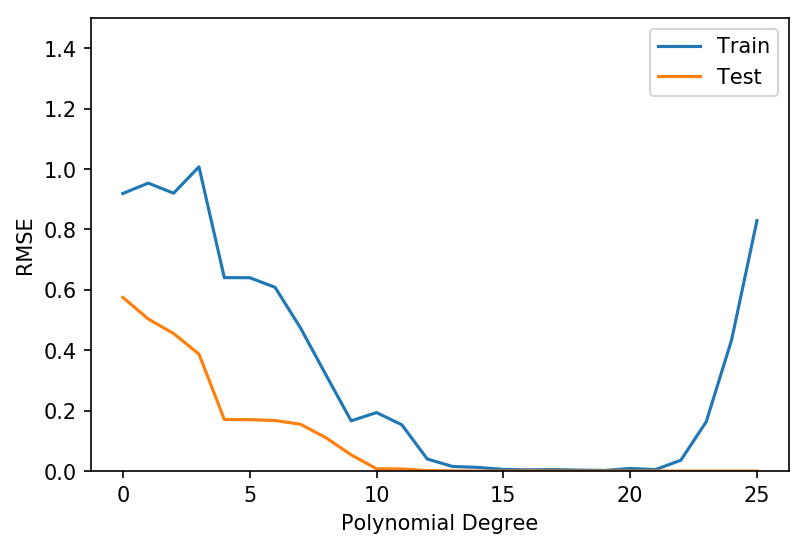
\includegraphics[width=0.6\linewidth]{pictures/polynomial_regression_our_version_degree_26.png}
	\centering
	\caption{Plotting the error for all different Polynomials using np.linalg.pinv for the pseudo-inverse. The minimum is still at degree 21.}
	\label{fig:pinv2}
\end{figure}
Unfortunately we start overfitting after degree 21. But it was good to check nonetheless. It is also worth noting that the graphs for the version using the ridge coefficient \ref{fig:ridge} and the graph showing the RMSE for the np.linalg.pinv versions \ref{fig:pinv1} and \ref{fig:pinv2} have the same behavior up to a polynom of 9th degree. After that the SVD version outperforms the ridge version with an RMSE of 0.00491 on the test data for a polynom of degree 21.

For the sake of futher comparision we plot the data and the predictions made by our new model. \ref{fig:pinv3}. In comparison the RMSE from the ridge version with 0.08899 is about 18 times bigger, than the RMSE from SVD, however in actual comparision one can argue that the effect of using SVD doesn't perform 18 times better than ridge. 
\begin{figure}[H]
	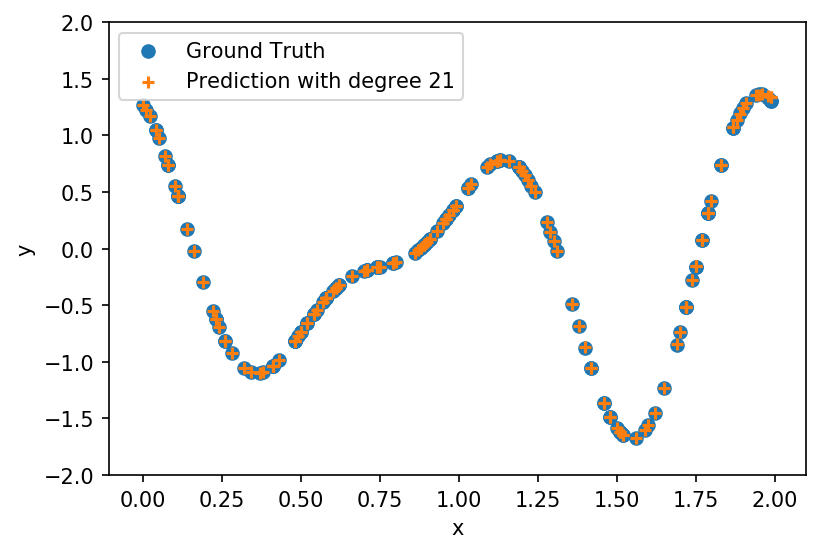
\includegraphics[width=0.6\linewidth]{pictures/groundTruth_polynomial_21.png}
	\centering
	\caption{The dataset and the predictions by our model. Even on test data the error is very small}
	\label{fig:pinv3}
\end{figure}

Finally lets have a look at some of the used source code. Depending on which version shall be used either line 25 or 27+28 needs to be commented out.
\lstinputlisting[language=Python]{code/polyReg.py}

\end{question}

%----------------------------------------------

\begin{question}{Gaussian Features}{4}
Now use Gaussian features. Each feature is a Gaussian distribution were the means are distributed linearly in $x \in[0,2]$ and the variance is set to $\sigma^2=0.02$. The features have to be normalized, i.e., they have to sum to one at every $x$. Using 10 features generate a plot with the activation of each feature over time (i.e., plot the matrix $\Phi$). Attach a snippet of your code showing how to compute Gaussian features.

\begin{answer}
Lets have a look at the matrix Phi using 10 Gaussian Features. Since they're all normalized to sum up to one at every point the gaussians at the edge have bigger values.
\end{answer}
\begin{figure}[H]
	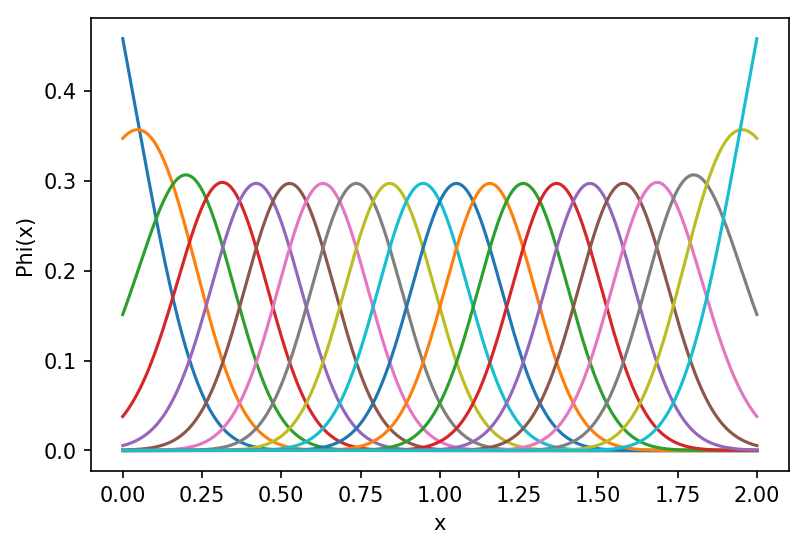
\includegraphics[width=0.7\linewidth]{pictures/Phi.png}
	\centering
	\caption{The Design Matrix using 10 Gaussian Features with mean set between 0 and 2.}
	\label{fig:phi}
\end{figure}

\lstinputlisting[language=Python]{code/gausReg.py}
\end{question}

%----------------------------------------------

\begin{question}{Gaussian Features, Continued}{4}
Repeat the process of fitting the model using the Gaussian features from the previous question. Compare the RMSE on the testing data using $15 \ldots 40$ basis functions and plot the RMSE. Which number of basis functions has the best performance and what is the best RMSE? Use a ridge coefficient of $\lambda=10^{-6}$.

\begin{answer}\end{answer}
We start by trying out all the given numbers of gaussian features and plot the results. The smalles error (RMSE = 0.01543) is given by using 29 gaussian features \ref{fig:numberGaus}. In the context of our findings in the last questions its interesting to note, that switching the method of calculating the pseudo inverse using gaussian features does not result in different metrics. Meaning that both methods evaluated in the last questions yield the same result. Hence we will use the ridge version. 
\begin{figure}[H]
	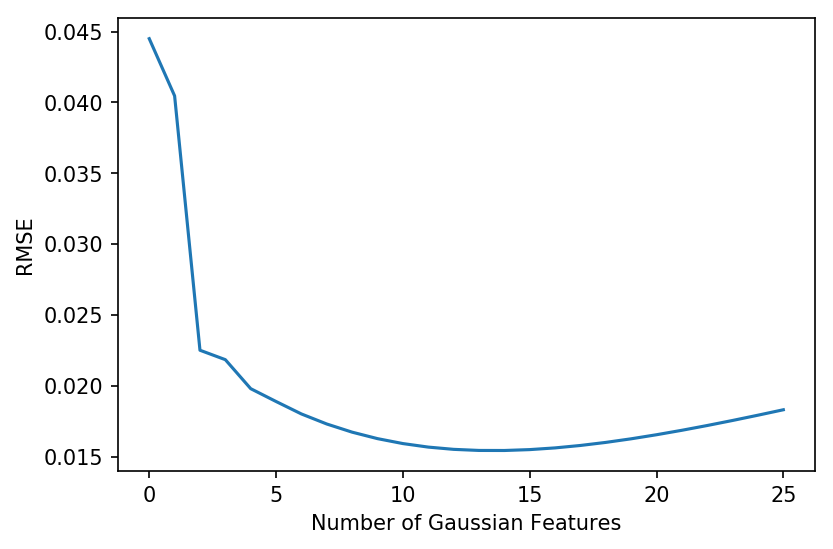
\includegraphics[width=0.6\linewidth]{pictures/number_of_gaussian.png}
	\centering
	\caption{Comparing the number of different gaussian features used, we get that 29 functions perform best.}
	\label{fig:numberGaus}
\end{figure}

When looking at the actual predictions made by the model we see that it performs better than the polynomial regression using ridge coefficient, but slightly worse than the polynomial regression using SVD.

When plotting the ground truth and predictions of this model, we see similar performance to polynomial regression with SVD \ref{fig:gaus29}.
\begin{figure}[H]
	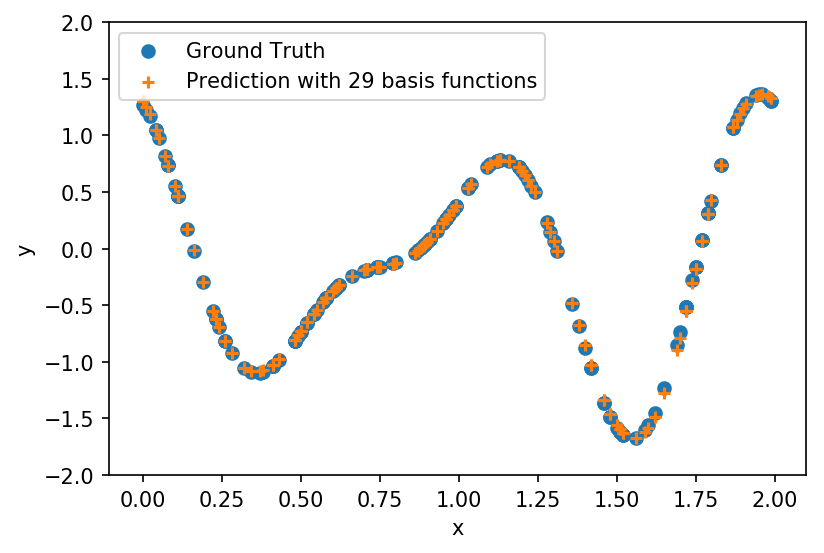
\includegraphics[width=0.5\linewidth]{pictures/groundTruth_gaus_29.png}
	\centering
	\caption{Comparing the actual data with the one produced by the model we get farily good results using gaussian features (RMSE=0.01543).}
	\label{fig:gaus29}
\end{figure}

\end{question}

%----------------------------------------------

\begin{question}{Bayesian Linear Regression}{10}
Using Bayesian linear regression, plot the mean and the standard deviation of the predictive distribution learned using the first $\{10, 12, 16, 20, 50, 150\}$ data points (one plot per case; plot it in the interval $x\in[0,2]$).
Discuss how the model uncertainty changes with the amount of data points and the problem of overfitting with Bayesian linear regression.
Use the best performing polynomial features that you found in 3.1a, a ridge coefficient of $\lambda=10^{-6}$, and assume Gaussian noise with $\sigma^2=0.0025$. 

\begin{answer}\end{answer}
\end{question}

%----------------------------------------------

\begin{question}[bonus]{Cross Validation}{5}
So far, we have split our dataset in two sets: training data and testing data. Cross-validation is a more sophisticated approach for model selection. Discuss it and its variants, pointing out their pro and cons.
\end{question}


Cross validation is used for a number of different techniques in machine learning. In general it means comparing a Trainingset with some kind of Validation or Testset. Using this definition the easiest crossvalidation-method is the holdout method. The holdout method splits the data into three sets: Training-, Validation and Testset. The machine learning Algorithm is trained using the training set and evaluated on the validation set, for tweaking the parameters\ref{fig:holdout}. This approach prevents knowledge "leaking" from the Testset into the model. Therefore the metrics used on the testing set will measure the ability of the model to generalize. 
\begin{figure}[H]
	\includegraphics[width=0.7\linewidth]{pictures/holdout.png}
	\centering
	\caption{Holdout Cross-Validation schematic}
	\label{fig:holdout}
\end{figure}



While simple, this approach comes with several limitations. Mainly in reducing the number of training samples for learning the model drastically, but also for introducing a high amount of variance in the evaluation, since the results can depend on a particular random choice of train and validation sets. 

To solve this problem k-fold crossvalidation (often just cross-validation, cv) is used. A test set still needs to be hold out for final validation, but we dont need a seperate validation set anymore. Instead we split the training set in \textit{k} smaller sets. The model is now trained on k-1 sets and validated on the remaining part. This process is now repeated for each of the "k-folds" \ref{fig:holdout}.

\begin{figure}[H]
	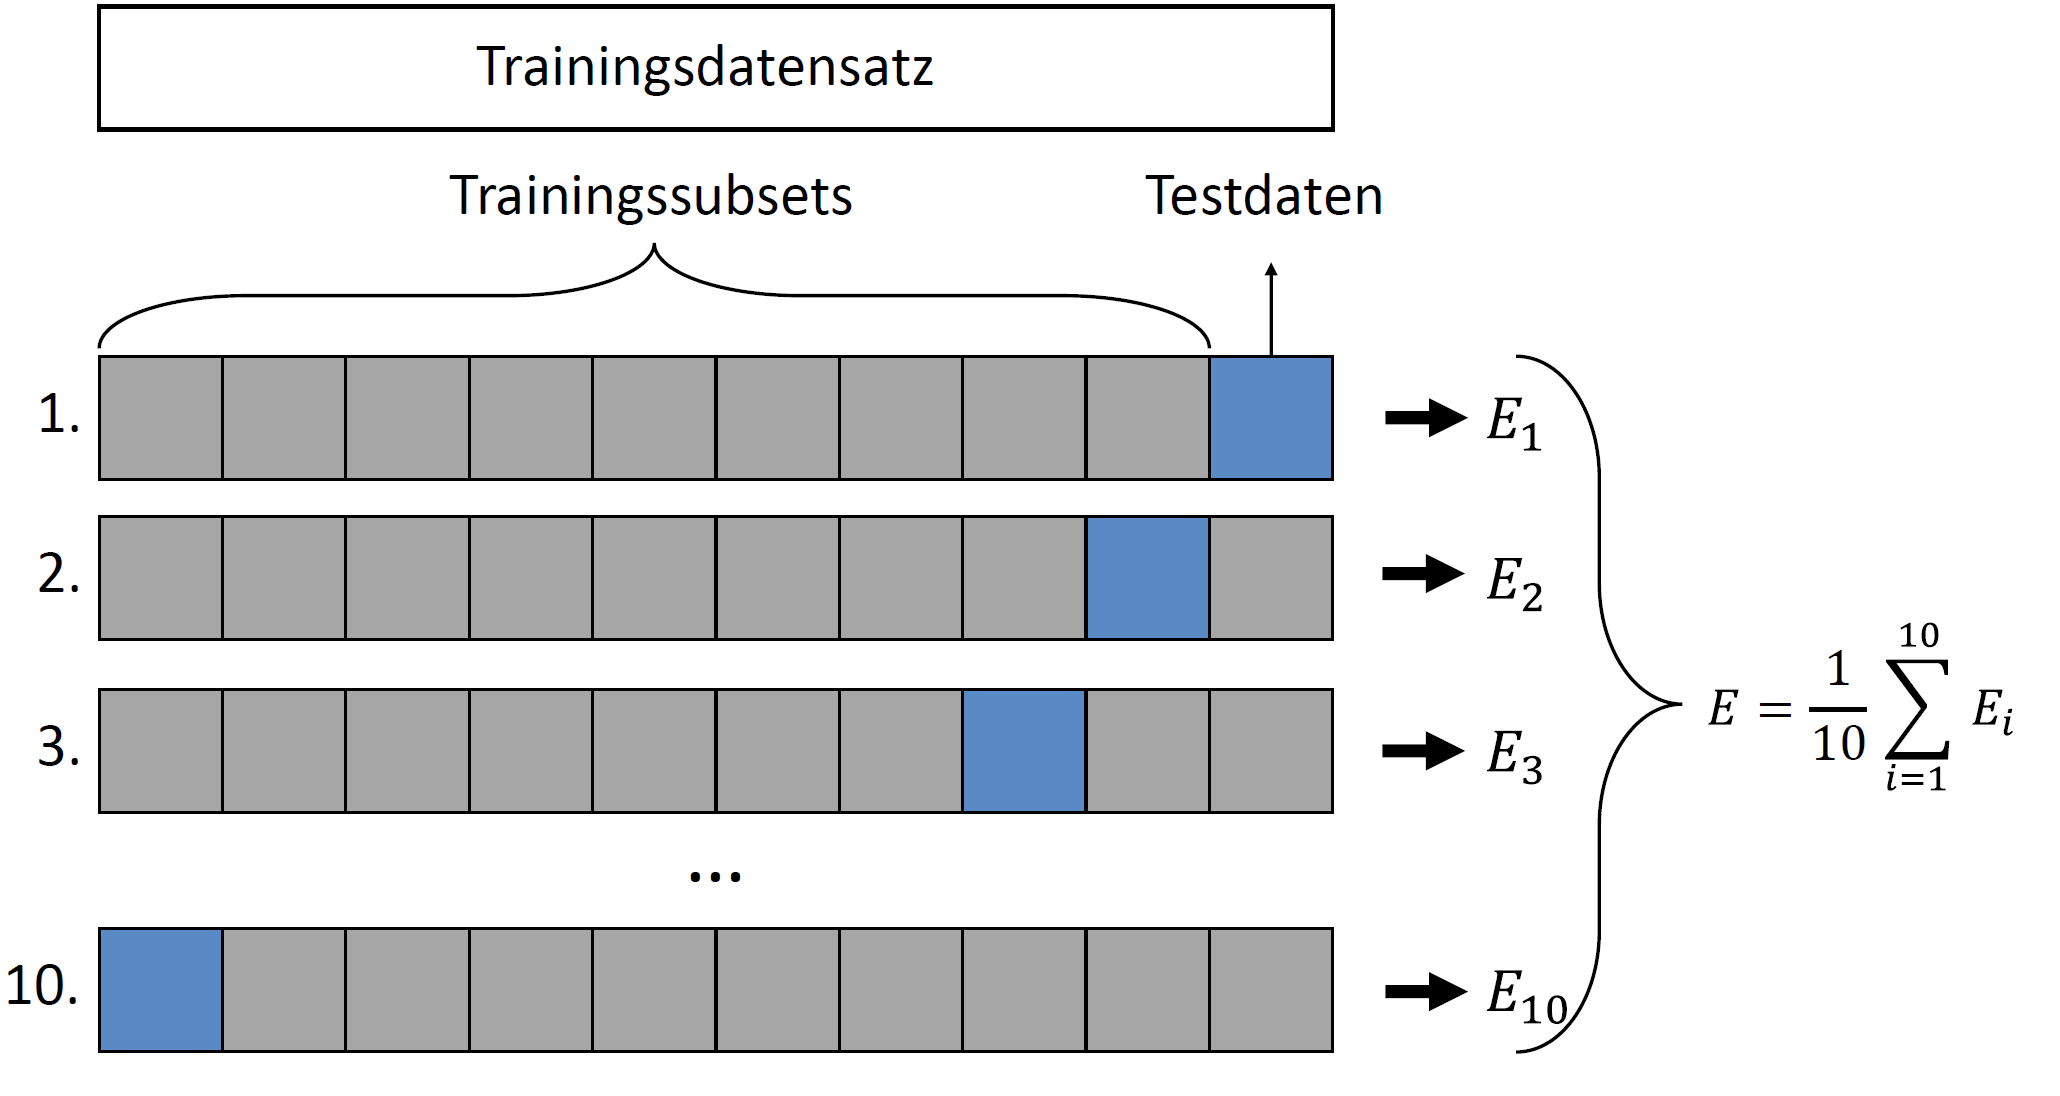
\includegraphics[width=0.7\linewidth]{pictures/cross_validation.png}
	\centering
	\caption{k-Fold cross validation splits the data into k-sets.}
	\label{fig:cv}
\end{figure}

The measured perfromance is the average of all individuall runs. This approach can be quite expensive to compute, but uses less data and generally leads to less variance in the outcome. 

To futher reduce the variance one can use the stratified k-fold cross-validation method. This method can be used, whenever all data is seen as equally important by the estimator, but may not be in reality. Instead of random shuffling the datasets, the stratified approach tries to create "stratified" folds, meaning that all folds have about the same percentage of samples of each target class, as the complete set. Only works on classification problems. 

K-fold cross-validation reaches its limiations when one wants to Hyperparameterize their models. Since no validation set is used, any change of parameters done after seeing the test metrics will lead to overfitting. To bypass this, nested cross-validation is used. In nested cross-validation another loop is added to the process, to be able to hyperparameterize algorithms. Now the inner cross-validation loop is used for training and validating models, while the outer loop is used for changing hyperparameters (for example by using grid search) and to evaluate different model architectures. For example, when using nested cross-validation with neural networks, the inner loop is used to train the network by changing its weights and bias vectors and validate its generalizing performance. Meanwhile the outer loop will be used for changing its hyperparameters e.g. the number of hidden layers and Neurons. The result of the outer loop leads to the best overall model. The excact process is shown in the picture \ref{fig:ncv}.

\begin{figure}[H]
	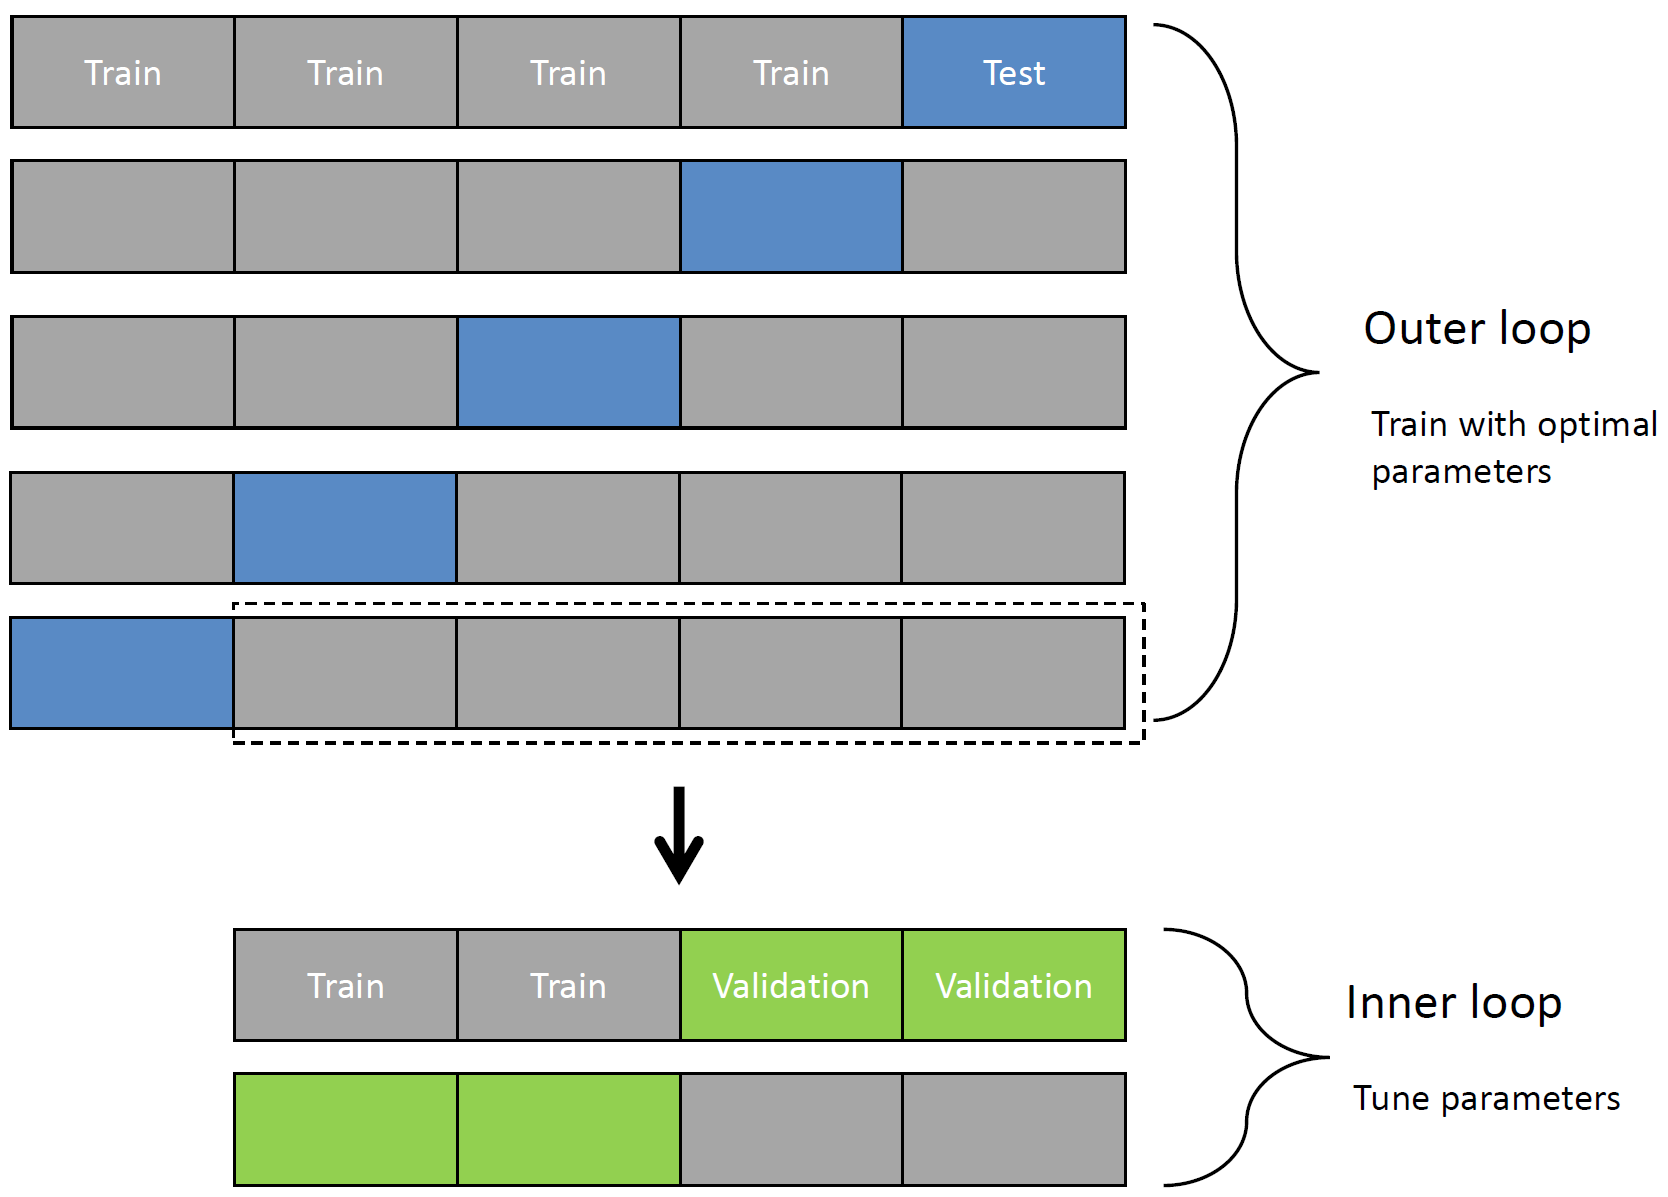
\includegraphics[width=0.8\linewidth]{pictures/nested_cross_validation.png}
	\centering
	\caption{Schematic of nested cross validation. The inner loop is used to train and validate a simple mode, while the outer loop is used to compare different model architecures.}
	\label{fig:ncv}
\end{figure}

\begin{answer}
\end{answer}

\end{questions}
